\documentclass[12pt,a4paper]{article}
\usepackage[utf8]{inputenc}
\usepackage[english]{babel}
\usepackage{geometry}
\geometry{a4paper, left=3cm, right=2cm, top=2.5cm, bottom=2.5cm} 
\usepackage{graphicx} 
\usepackage{hyperref}
\usepackage{xcolor}
\usepackage{tabularx}
\usepackage{booktabs}
\usepackage{float}
\usepackage{amsmath}
\usepackage{titlesec}
\usepackage{enumitem}
\usepackage{tikz} 
\usetikzlibrary{calc, shapes.geometric, arrows.meta, positioning}
\usepackage{listings}
\usepackage{xcolor}

\usepackage{mathpazo} 
\usepackage{microtype} 
\usepackage{setspace} 
\setstretch{1.15} 

\lstdefinestyle{pythonstyle}{
    backgroundcolor=\color{gray!8},
    commentstyle=\color{gray!60!black}\itshape,
    keywordstyle=\color{blue!70!black}\bfseries,
    stringstyle=\color{orange!80!black},
    basicstyle=\ttfamily\small,
    breakatwhitespace=false,
    breaklines=true,
    keepspaces=true,
    numbers=left,
    numbersep=8pt,
    numberstyle=\tiny\color{gray},
    showspaces=false,
    showstringspaces=false,
    showtabs=false,
    tabsize=4,
    frame=single,
    rulecolor=\color{gray!40},
    xleftmargin=15pt,
    xrightmargin=5pt,
}
\lstset{style=pythonstyle}

\begin{document}

\newgeometry{top=2.3cm, left=3cm, right=2cm, bottom=2.5cm}
\begin{titlepage}
    \begin{tikzpicture}[remember picture, overlay]
        \draw[line width = 2pt] ($(current page.north west) + (2.5cm,-2cm)$) rectangle ($(current page.south east) + (-1.5cm,2cm)$);
        \draw[line width = 0.5pt] ($(current page.north west) + (2.6cm,-2.1cm)$) rectangle ($(current page.south east) + (-1.6cm,2.1cm)$);
    \end{tikzpicture}
    \centering
    \singlespacing
    \resizebox{0.95\textwidth}{!}{\textbf{HANOI UNIVERSITY OF SCIENCE AND TECHNOLOGY}}\\[0.8cm]
    \resizebox{0.95\textwidth}{!}{\textbf{School of Information and Communication Technology}}\\[1.8cm]
    
\includegraphics[width=0.25\textwidth]{hust-logo.png}\\[1.8cm]
    {\huge \textbf{TECHNICAL REPORT}}\\[1.2cm]
    {\LARGE \textbf{USING MACHINE LEARNING TO\\[0.3cm] DETECT MALICIOUS LINKS}}\\[1cm]
    \vfill
    \begin{flushleft}
        \large
        \hspace{2.5cm} 
        \begin{tabular}{ll}
            \textbf{Project:} & Cyberspace Safety Assessment \\[0.3cm]
            \textbf{Document:} & Architecture and Specification \\[0.3cm]
            \textbf{Instructor:} & Tran Duc Duy \\[0.3cm]
            \textbf{Student:} & Do Thanh Trung - 202416833 \\[0.3cm]
            \textbf{Date:} & June 2026
        \end{tabular}
    \end{flushleft}
    \vspace*{2cm}
\end{titlepage}
\restoregeometry

\newpage
\begin{spacing}{1.1}
\tableofcontents
\end{spacing}
\newpage

%% ============================================================
\section{System Overview}
%% ============================================================

Detecting phishing websites is a classic yet ever-evolving challenge in the field of Information Security. Traditional methods, such as utilizing blacklists (e.g., Google Safe Browsing), suffer from a fatal flaw: high latency and the inability to detect Zero-day attacks (newly generated malicious URLs).

This system is designed to overcome these limitations by combining \textbf{Heuristic Analysis} with \textbf{Ensemble Machine Learning}. Unlike content-based analysis systems that require fetching HTML/JavaScript, this system performs \textbf{Lexical Analysis}---analyzing solely the structure of the URL string. This approach ensures ultra-fast response times, making it highly suitable for real-time API integration.

%% ============================================================
\section{Training Data Sources}
%% ============================================================

The success of a Machine Learning model heavily depends on the quality and coverage of its training dataset. To ensure the system can identify a wide range of global attack vectors while remaining optimized for the Vietnamese cyberspace, the dataset was aggregated and pre-processed from three primary sources:

\subsection{International Dataset (Kaggle) and Label Aggregation}
The core data was extracted from the public \textbf{``Malicious URLs dataset''} on Kaggle (authored by \textit{sid321axn}). Originally, this dataset provides hundreds of thousands of URL samples structured as a multi-class classification problem with four distinct morphological labels:
\begin{itemize}
    \item \textbf{Benign:} Safe and legitimate websites.
    \item \textbf{Phishing:} Fraudulent websites designed to steal credentials.
    \item \textbf{Malware:} Links used to distribute malicious software.
    \item \textbf{Defacement:} Legitimate websites that have been compromised and altered by hackers.
\end{itemize}

However, to align with the core objective of the project---which is to provide a decisive, real-time warning to end-users (Safe vs.\ Dangerous)---we implemented a \textbf{Binary Label Aggregation} strategy. All malicious sub-categories (\textit{Phishing, Malware, Defacement}) were merged into a single positive class labeled as \texttt{1} (Dangerous), while \textit{Benign} remained as class \texttt{0} (Safe).

This approach not only simplifies the decision boundary for Tree-based models (XGBoost and Random Forest) but also significantly reduces noise and class imbalance issues during the training phase, thereby maximizing the model's recall rate for any type of cyber threat.

\subsection{Vietnam-Specific Dataset (Tin Nhiem Mang)}
A common drawback of international datasets is the omission of targeted phishing campaigns aimed specifically at Vietnamese users. To address this, the development team performed automated data collection from the \textbf{Tin Nhiem Mang} project (\url{tinnhiemmang.vn}), operated by the National Cyber Security Center (NCSC) of Vietnam.

By integrating this localized dataset, the system learned to recognize the structural patterns of legitimate Vietnamese entities (\texttt{.gov.vn}, \texttt{.edu.vn}) while effectively identifying spoofed domestic brands (e.g., local banks and e-commerce platforms).

\subsection{Global Whitelist (Tranco List)}
Furthermore, to ensure the model correctly identifies a wide spectrum of legitimate international websites and avoids bias (False Positives), we constructed an extensive \textbf{Global Whitelist} using data from the \textbf{Tranco List}.

The Tranco dataset provides a highly reliable, research-grade ranking of the top millions of websites globally. By incorporating a subset of these top-ranking domains into our training pipeline, the model achieved a robust understanding of benign URL structures at an international scale, effectively balancing the aggressive detection of the heuristic rules.

%% ============================================================
\section{Processing Pipeline}
%% ============================================================

The system processes an input URL through five sequential defense layers:
\begin{enumerate}
    \item \textbf{Shortener Pre-Check:} Detects URL shortening services before any whitelist bypass.
    \item \textbf{Whitelist Check:} Bypasses further inspection for known reputable domains.
    \item \textbf{Hard Rules:} Handles explicitly malicious behaviors with deterministic verdicts.
    \item \textbf{ML Ensemble:} Analyzes URL features using XGBoost, LightGBM, Random Forest, \& Logistic Regression.
    \item \textbf{Dynamic Thresholding:} Adjusts sensitivity based on camouflage techniques and domain context.
\end{enumerate}

\begin{figure}[H]
    \centering
    \resizebox{0.85\textwidth}{!}{
    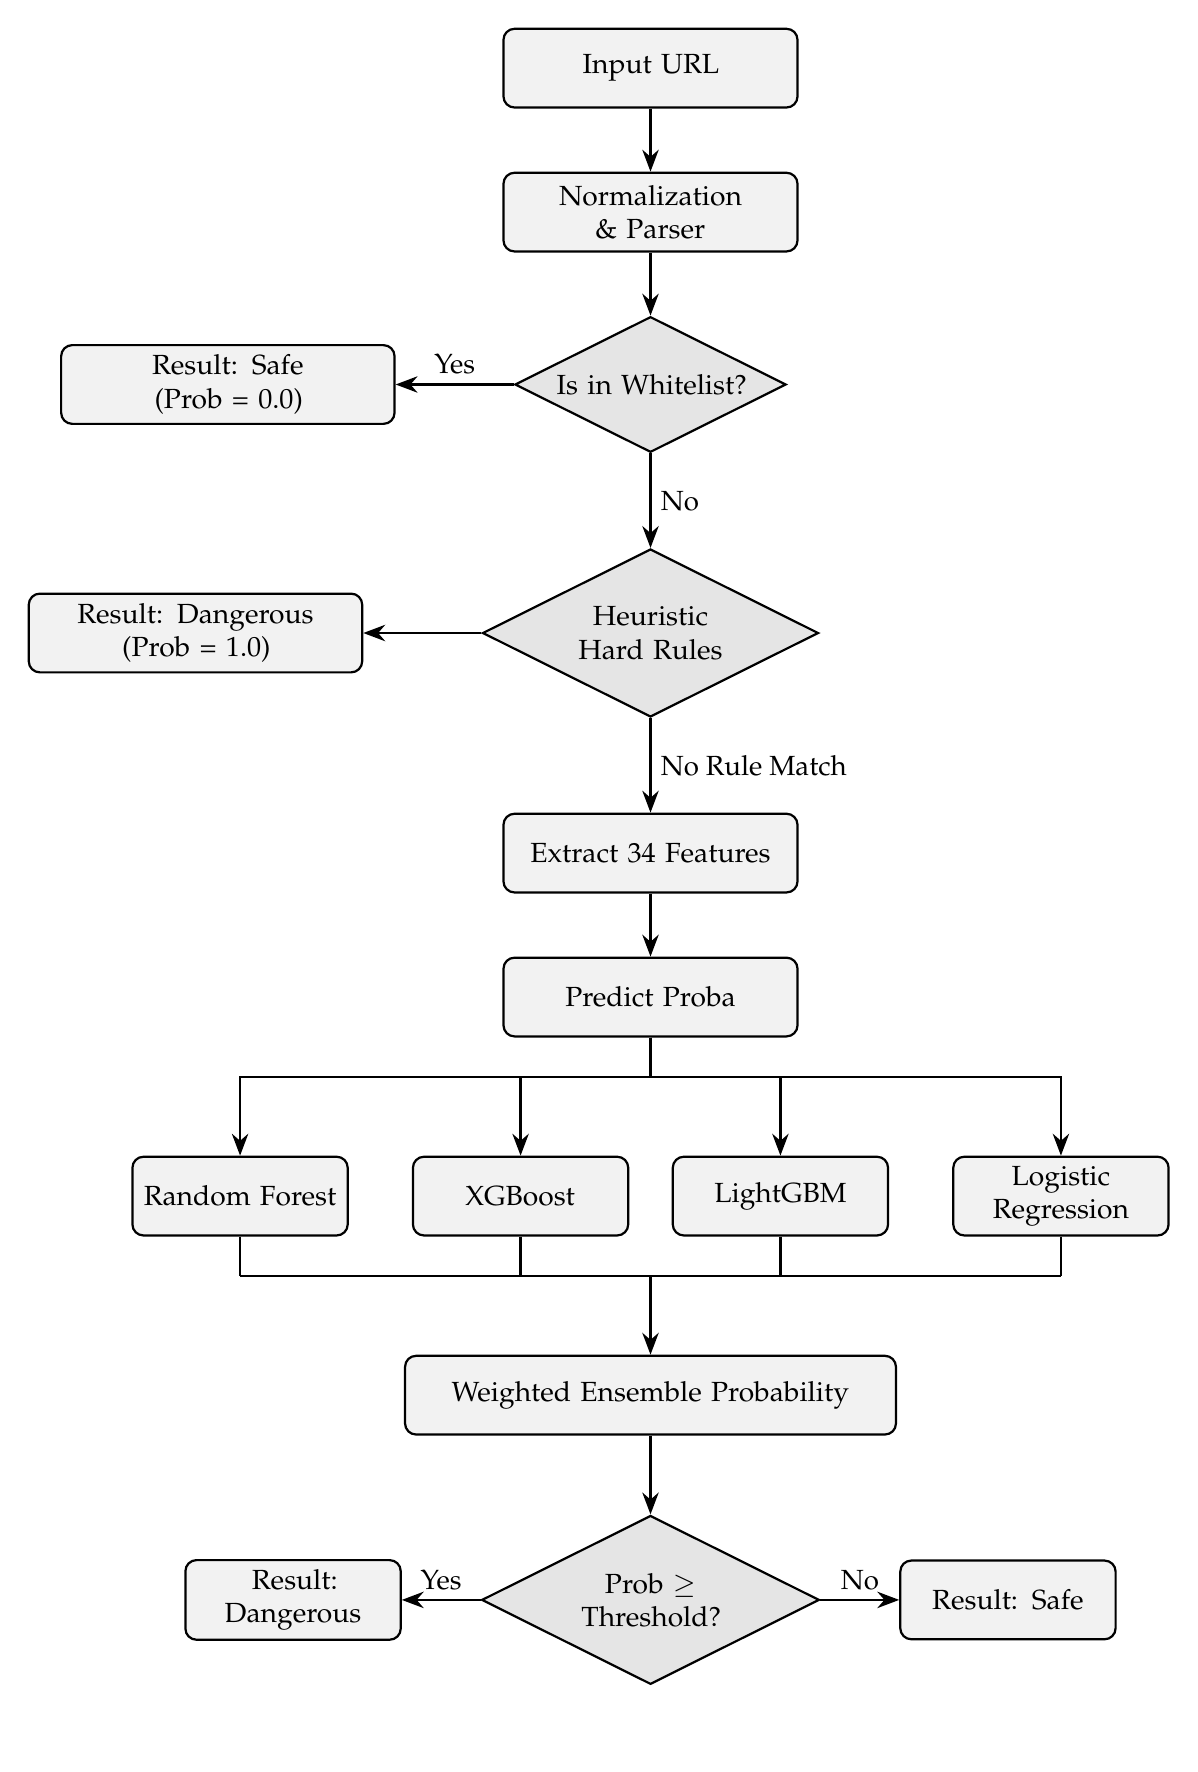
\begin{tikzpicture}[
        node distance=1.5cm and 2cm,
        box/.style={rectangle, draw=black, thick, fill=gray!10, text width=3.5cm, align=center, minimum height=1cm, rounded corners},
        decision/.style={diamond, aspect=2, draw=black, thick, fill=gray!20, text width=2.5cm, align=center, inner sep=2pt},
        arrow/.style={-{Stealth[scale=1.2]}, thick}
    ]
        % Nodes
        \node[box] (input) {Input URL};
        \node[box, below=0.8cm of input] (norm) {Normalization \& Parser};
        \node[decision, below=0.8cm of norm] (whitelist) {Is in Whitelist?};
        
        \node[box, left=1.5cm of whitelist, text width=4cm] (safe1) {Result: Safe\\(Prob = 0.0)};
        
        \node[decision, below=1.2cm of whitelist] (rules) {Heuristic Hard Rules};
        
        \node[box, left=1.5cm of rules, text width=4cm] (danger1) {Result: Dangerous\\(Prob = 1.0)};
        
        \node[box, below=1.2cm of rules] (extract) {Extract 34 Features};
        
        \node[box, below=0.8cm of extract] (predict) {Predict Proba};
        
        \node[box, below=1.5cm of predict, xshift=-1.65cm, text width=2.5cm] (xgb) {XGBoost};
        \node[box, below=1.5cm of predict, xshift=1.65cm, text width=2.5cm] (lgb) {LightGBM};
        \node[box, left=0.8cm of xgb, text width=2.5cm] (rf) {Random Forest};
        \node[box, right=0.8cm of lgb, text width=2.5cm] (lr) {Logistic\\Regression};
        
        \node[box, below=1.5cm of xgb, xshift=1.65cm, text width=6cm] (ensemble) {Weighted Ensemble Probability};
        
        \node[decision, below=1cm of ensemble] (thresh) {Prob $\geq$ Threshold?};
        
        \node[box, left=1cm of thresh, text width=2.5cm] (danger2) {Result: Dangerous};
        \node[box, right=1cm of thresh, text width=2.5cm] (safe2) {Result: Safe};
        
        % Arrows
        \draw[arrow] (input) -- (norm);
        \draw[arrow] (norm) -- (whitelist);
        \draw[arrow] (whitelist) -- node[above] {Yes} (safe1);
        \draw[arrow] (whitelist) -- node[right] {No} (rules);
        
        \path (rules) -- coordinate[midway] (mid1) (danger1);
        \node[above=0.1cm of mid1, align=center, font=\small] {};
        \draw[arrow] (rules) -- (danger1);
        
        \draw[arrow] (rules) -- node[right] {No Rule Match} (extract);
        
        \draw[arrow] (extract) -- (predict);
        
        \draw[arrow] (predict.south) -- ++(0,-0.5) -| (rf.north);
        \draw[arrow] (predict.south) -- ++(0,-0.5) -| (xgb.north);
        \draw[arrow] (predict.south) -- ++(0,-0.5) -| (lgb.north);
        \draw[arrow] (predict.south) -- ++(0,-0.5) -| (lr.north);
        
        \path (rf.south) ++(0,-0.5) coordinate (bus_y);
        \draw[thick] (rf.south) -- (rf.south |- bus_y) coordinate (b1);
        \draw[thick] (xgb.south) -- (xgb.south |- bus_y) coordinate (b2);
        \draw[thick] (lgb.south) -- (lgb.south |- bus_y) coordinate (b3);
        \draw[thick] (lr.south) -- (lr.south |- bus_y) coordinate (b4);
        \draw[thick] (b1) -- (b4);
        \draw[arrow] ($(b2)!0.5!(b3)$) -- (ensemble.north);
        
        \draw[arrow] (ensemble) -- (thresh);
        
        \draw[arrow] (thresh) -- node[above] {Yes} (danger2);
        \draw[arrow] (thresh) -- node[above] {No} (safe2);
        \node[below=0.5cm of thresh] (dummy) {}; % Dummy node for bottom padding
    \end{tikzpicture}
    }
    \vspace{0.2cm}
    \caption{Pipeline Architecture of the Detection System}
    \label{fig:pipeline}
\end{figure}

The entry point is the \texttt{predict\_single\_url()} function in \texttt{predict.py}. After normalizing the input (prepending \texttt{https://} if no scheme is present and stripping trailing slashes and \texttt{www.}), it delegates to the five layers in order. Below is the complete implementation:

\lstinputlisting[language=Python, caption={predict.py --- Full prediction pipeline (RF + XGB ensemble with hard rules)}, label={lst:predict}]{src/predict.py}

%% ============================================================
\section{Whitelist and Trusted Domain Resolution}
%% ============================================================

The first layer of the pipeline performs a whitelist check before any feature extraction takes place (with the exception of URL shortener detection, which runs even earlier). The \texttt{is\_trusted\_domain()} function in \texttt{feature.py} implements a two-tier trust resolution strategy.

\subsection{Tier 1 --- Static Whitelist}

The system maintains a hardcoded set of 27 high-confidence trusted domains (e.g., \texttt{google.com}, \texttt{facebook.com}, \texttt{vietcombank.com.vn}) supplemented by a dynamic whitelist loaded at startup from \texttt{data/whitelist.txt} (capped at 5,000 entries, generated from the Tranco Top-1M list). A hostname passes this tier if it exactly matches any whitelisted domain or is a subdomain thereof (suffix check).

\subsection{Tier 2 --- eTLD-Aware Brand Resolution via \texttt{tldextract}}

A critical edge case arises with country-code second-level TLDs (ccSLDs) such as \texttt{.co.uk}, \texttt{.com.vn}, and \texttt{.com.au}. A na\"ive suffix extraction would misidentify the SLD of \texttt{microsoft.co.uk} as \texttt{co} rather than \texttt{microsoft}, causing legitimate brand domains to fail the trust check.

The system handles this by delegating eTLD resolution to the \texttt{tldextract} library, which maintains an up-to-date copy of the Public Suffix List. Given a hostname, \texttt{tldextract.extract()} returns three components: \texttt{subdomain}, \texttt{domain} (SLD), and \texttt{suffix} (effective TLD). The trust check then verifies:

\begin{itemize}
    \item The extracted \texttt{domain} (SLD) is a member of the \texttt{FAMOUS\_BRANDS} set.
    \item The leaf label of the \texttt{suffix} (i.e., the rightmost TLD component) is \textit{not} in the \texttt{SUSPICIOUS\_TLDS} set.
\end{itemize}

\noindent If both conditions hold, the domain is granted full trust and the pipeline returns \texttt{safe} immediately.

\vspace{0.4cm}
\begin{table}[H]
    \centering
    \begin{tabularx}{\textwidth}{lllX}
        \toprule
        \textbf{Input Hostname} & \textbf{Extracted SLD} & \textbf{TLD} & \textbf{Trusted?} \\
        \midrule
        \texttt{microsoft.co.uk}    & \texttt{microsoft}   & \texttt{uk}  & Yes \\
        \texttt{vietcombank.com.vn} & \texttt{vietcombank} & \texttt{vn}  & Yes (static whitelist) \\
        \texttt{paypa1.com}         & \texttt{paypa1}      & \texttt{com} & No (not in \texttt{FAMOUS\_BRANDS}) \\
        \texttt{google.xyz}         & \texttt{google}      & \texttt{xyz} & No (TLD is suspicious) \\
        \bottomrule
    \end{tabularx}
    \caption{Examples of eTLD-aware brand resolution outcomes}
    \label{tab:whitelist_examples}
\end{table}

%% ============================================================
\section{Hard Rule Engine}
%% ============================================================

Before invoking the machine learning ensemble, the pipeline applies a deterministic rule engine that short-circuits evaluation and immediately returns \texttt{prediction = 1 (dangerous)} with \texttt{prob = 1.0} whenever a URL matches a known malicious pattern. These rules encode domain-expert knowledge that does not require probabilistic inference---if the condition is met, the verdict is certain.

There are seven independent rules, evaluated in order. The first match terminates the pipeline.

\subsection{Rule 0 --- URL Shortener Detection (Pre-Whitelist)}
\begin{center}
\texttt{hostname} $\in$ \texttt{SHORTENERS}
\end{center}
\noindent This rule runs \textit{before} the whitelist check. URL shortening services (e.g., \texttt{bit.ly}, \texttt{tinyurl.com}, \texttt{t.co}) are frequently abused to obscure malicious destinations. Even though some shorteners may appear in the Tranco Top-1M whitelist, any shortened URL is inherently suspicious because the final destination is hidden from the user. When triggered, the ML ensemble still runs to produce a probability score for informational purposes, but the \texttt{prediction} is forced to \texttt{1 (dangerous)} with the source marked as \texttt{hard\_rule}.

\subsection{Rule 1 --- Brand Spoofing (Normal TLD)}
\begin{center}
\texttt{brand\_similarity} $\geq 0.75$ \quad \textbf{AND} \quad \texttt{tld\_suspicious} $= 0$
\end{center}
\noindent A domain whose Second-Level Domain (SLD) is highly similar to a known brand name (similarity score $\geq 0.75$) \textit{and} which uses a legitimate, non-flagged TLD is almost certainly a spoofed site. The use of a reputable TLD (e.g., \texttt{.com}, \texttt{.net}) is itself a social engineering tactic designed to lower the victim's guard. Example: \texttt{paypa1.com}, \texttt{g00gle.net}.

\subsection{Rule 2 --- Brand Spoofing (Suspicious TLD)}
\begin{center}
\texttt{tld\_suspicious} $= 1$ \quad \textbf{AND} \quad \texttt{brand\_similarity} $\geq 0.65$
\end{center}
\noindent When the TLD already belongs to the suspicious set (e.g., \texttt{.xyz}, \texttt{.tk}, \texttt{.top}), the brand similarity threshold is relaxed from 0.75 down to 0.65. The rationale is that a suspicious TLD is itself a strong independent signal; even a moderate brand resemblance in this context is highly indicative of a phishing campaign. Example: \texttt{facebo0k.xyz}, \texttt{shopee-login.top}.

\subsection{Rule 3 --- C2 Server Callback Detection (Random Subdomain)}
\begin{center}
\texttt{has\_uuid\_path} $= 1$ \quad \textbf{AND} \quad \texttt{subdomain\_is\_random} $= 1$
\end{center}
\noindent Command-and-Control (C2) infrastructure used by malware often follows a characteristic pattern: a randomly generated subdomain (e.g., \texttt{euftrhnx}) paired with a UUID-formatted path segment (e.g., \texttt{/ba1019ee-a048-4bd5-a90d-1fc5da2b8696}). The subdomain provides Domain Generation Algorithm (DGA) evasion, while the UUID serves as a unique victim or session identifier. Flagging both signals simultaneously yields a near-zero false positive rate for this class of threat.

\subsection{Rule 4 --- C2 Server Callback Detection (High-Entropy Subdomain)}
\begin{center}
\texttt{has\_uuid\_path} $= 1$ \quad \textbf{AND} \quad \texttt{subdomain\_entropy} $\geq 2.4$
\end{center}
\noindent This rule is a fallback for Rule~3 that catches C2 patterns where the \texttt{subdomain\_is\_random} heuristic may not fire (e.g., subdomains with some vowels but still machine-generated). A UUID in the path combined with high Shannon entropy in the subdomain remains a strong indicator of automated C2 infrastructure.

\subsection{Rule 5 --- Executable Distribution via Random Subdomain}
\begin{center}
\texttt{has\_executable\_ext} $= 1$ \quad \textbf{AND} \quad \texttt{subdomain\_is\_random} $= 1$
\end{center}
\noindent URLs that serve executable file types (\texttt{.exe}, \texttt{.msi}, \texttt{.apk}, \texttt{.sh}, etc.) from domains with machine-generated subdomains are strong indicators of malware distribution from compromised or ephemeral VPS infrastructure.

\subsection{Rule 6 --- Executable Distribution via Free Hosting}
\begin{center}
\texttt{has\_executable\_ext} $= 1$ \quad \textbf{AND} \quad \texttt{is\_free\_hosting} $= 1$
\end{center}
\noindent Legitimate software vendors do not distribute executables from free developer hosting platforms (e.g., \texttt{vercel.app}, \texttt{netlify.app}, \texttt{github.io}). This combination is almost exclusively associated with malware dropper campaigns.

\subsection{Rule 7 --- Malware Distribution via Free Hosting}
\begin{center}
\texttt{free\_hosting\_download} $= 1$
\end{center}
\noindent This is a composite feature (see Section~\ref{sec:features}) that fires when a URL is hosted on a free platform \textit{and} the path or query string contains a download or installation keyword. This pattern is strongly associated with malware dropper campaigns.

\vspace{0.4cm}
\begin{table}[H]
    \centering
    \begin{tabularx}{\textwidth}{llX}
        \toprule
        \textbf{Rule} & \textbf{Condition} & \textbf{Threat Class} \\
        \midrule
        0 & Hostname in \texttt{SHORTENERS}                       & Obfuscated destination (pre-whitelist) \\
        1 & \texttt{brand\_sim} $\geq 0.75$ + non-suspicious TLD  & Phishing (brand spoof, trusted-looking domain) \\
        2 & \texttt{tld\_suspicious} + \texttt{brand\_sim} $\geq 0.65$ & Phishing (brand spoof, low-quality domain) \\
        3 & UUID path + random subdomain                          & Malware C2 callback / DGA \\
        4 & UUID path + subdomain entropy $\geq 2.4$              & Malware C2 callback (fallback) \\
        5 & Executable extension + random subdomain               & Malware distribution (random VPS) \\
        6 & Executable extension + free hosting                   & Malware distribution (free platform) \\
        7 & Free hosting + download/install in path               & Malware dropper distribution \\
        \bottomrule
    \end{tabularx}
    \caption{Summary of hard rule conditions and corresponding threat classes}
    \label{tab:hard_rules}
\end{table}

%% ============================================================
\section{Feature Engineering}
\label{sec:features}
%% ============================================================

The system extracts 34 numerical features from each URL using purely lexical analysis---no DNS resolution, no HTTP request, no HTML parsing. All features are computed solely from the URL string by the \texttt{extracting\_features()} function in \texttt{feature.py}. This ensures sub-millisecond feature extraction and eliminates any external dependency. The full implementation is listed below:

\lstinputlisting[language=Python, caption={feature.py --- Feature extraction and domain trust resolution}, label={lst:feature}]{src/feature.py}

\noindent Features are grouped into five categories described in the following subsections.

\subsection{Structural \& Length Features}

These features capture the overall morphology of the URL and are strong baseline signals for randomness or obfuscation:

\begin{table}[H]
    \centering
    \begin{tabularx}{\textwidth}{l >{\raggedright\arraybackslash}X}
        \toprule
        \textbf{Feature} & \textbf{Description} \\
        \midrule
        \texttt{url\_len}          & Total character length of the cleaned URL (scheme and \texttt{www.} stripped). \\
        \addlinespace[4pt]
        \texttt{domain\_len}       & Length of the \texttt{netloc} component (\textit{hostname:port}). \\
        \addlinespace[4pt]
        \texttt{path\_len}         & Length of the URL path component. \\
        \addlinespace[4pt]
        \texttt{count\_dot}        & Number of dots in the full URL (proxy for subdomain depth and TLD complexity). \\
        \addlinespace[4pt]
        \texttt{count\_hyphen}     & Number of hyphens; brand-spoof domains commonly insert hyphens (e.g., \texttt{paypal-secure.com}). \\
        \addlinespace[4pt]
        \texttt{count\_at}         & Presence of \texttt{@} in the URL; used to embed credentials before the real hostname. \\
        \addlinespace[4pt]
        \texttt{count\_slash}      & Slash count; deep paths are common in obfuscated redirect chains. \\
        \addlinespace[4pt]
        \texttt{count\_question}   & Number of \texttt{?} characters. \\
        \addlinespace[4pt]
        \texttt{count\_equal}      & Number of \texttt{=} characters (query parameter count proxy). \\
        \addlinespace[4pt]
        \texttt{count\_percent}    & Number of \texttt{\%} characters; high values indicate heavy URL encoding / obfuscation. \\
        \addlinespace[4pt]
        \texttt{count\_ampersand}  & Number of \texttt{\&} separators in the query string (parameter count). \\
        \addlinespace[4pt]
        \texttt{path\_depth}       & Number of \texttt{/} in the path; deep paths are unusual for legitimate landing pages. \\
        \addlinespace[4pt]
        \texttt{has\_port}         & Binary flag; non-standard ports (e.g., \texttt{:8080}) are uncommon for legitimate sites. \\
        \addlinespace[4pt]
        \texttt{is\_domain\_only}  & Binary flag; set to 1 when the URL is a bare domain with no path and no query string. Helps the model learn that bare domains with clean signals are generally safe. \\
        \bottomrule
    \end{tabularx}
    \caption{Structural and length features}
    \label{tab:feat_structural}
\end{table}

\subsection{Statistical \& Entropy Features}

These features quantify the degree of randomness and character distribution within the URL. High entropy is a reliable proxy for machine-generated strings---a common property of DGA-based domains and obfuscated phishing hostnames---while digit and letter ratios expose structural anomalies that deviate from naturally readable domain names.

\begin{table}[H]
    \centering
    \begin{tabularx}{\textwidth}{l >{\raggedright\arraybackslash}X}
        \toprule
        \textbf{Feature} & \textbf{Description} \\
        \midrule
        \texttt{shannon\_entropy}    & Shannon entropy $H = -\sum p_i \log_2 p_i$ computed over the hostname characters. High entropy (typically $> 3.5$) indicates a randomly generated string. \\
        \addlinespace[4pt]
        \texttt{subdomain\_entropy}  & Entropy computed \textit{exclusively} on the subdomain component (everything before \texttt{SLD.TLD}), isolating the random-subdomain signal without dilution from the base domain. \\
        \addlinespace[4pt]
        \texttt{digit\_ratio}        & Ratio of digit characters to total characters in the full URL. \\
        \addlinespace[4pt]
        \texttt{letter\_ratio}       & Ratio of alphabetic characters to total characters. \\
        \addlinespace[4pt]
        \texttt{domain\_digit\_count}& Absolute count of digits in the hostname. \\
        \addlinespace[4pt]
        \texttt{consecutive\_digits} & Binary flag for 4+ consecutive digits in the hostname (e.g., \texttt{192login.com}). \\
        \addlinespace[4pt]
        \texttt{path\_digit\_ratio}  & Ratio of digits to total characters in the path component. \\
        \bottomrule
    \end{tabularx}
    \caption{Statistical and entropy features}
    \label{tab:feat_entropy}
\end{table}

\subsection{Lexical \& Heuristic Features}

These features encode domain-expert knowledge about the vocabulary and structure of malicious URLs. Unlike the statistical group, they rely on curated reference sets---known bad TLDs, social-engineering keywords, famous brand names, and URL shortener hostnames---to produce binary signals that are both highly interpretable and computationally inexpensive.

\begin{table}[H]
    \centering
    \begin{tabularx}{\textwidth}{l >{\raggedright\arraybackslash}X}
        \toprule
        \textbf{Feature} & \textbf{Description} \\
        \midrule
        \texttt{tld\_suspicious}        & Binary flag; TLD membership in a curated set of high-abuse TLDs spanning generic abuse domains (\texttt{.tk}, \texttt{.xyz}, \texttt{.top}, \texttt{.icu}), gambling-related TLDs (\texttt{.bet}, \texttt{.casino}, \texttt{.poker}), and sport-themed TLDs (\texttt{.football}, \texttt{.cricket}, \texttt{.golf}). \\
        \addlinespace[4pt]
        \texttt{has\_suspicious\_word}  & Binary flag; URL contains any of 15 social-engineering keywords (e.g., \texttt{login}, \texttt{verify}, \texttt{password}, \texttt{prize}). \\
        \addlinespace[4pt]
        \texttt{has\_hex\_chars}        & Binary flag for more than 2 percent-encoded sequences (\texttt{\%XX}); indicates character-level obfuscation. \\
        \addlinespace[4pt]
        \texttt{is\_ip}                 & Binary flag; hostname matches an IPv4 address pattern. Legitimate services never use raw IPs as their primary URL. \\
        \addlinespace[4pt]
        \texttt{subdomain\_count}       & Number of subdomain levels above the SLD. \\
        \addlinespace[4pt]
        \texttt{brand\_similarity}      & Maximum fuzzy similarity score (0--1) between the SLD and any of 26 tracked brand names. The function first checks if the SLD \textit{contains} a brand name as a substring (returning 0.85 if so), then falls back to the average of \texttt{fuzz.ratio} and \texttt{fuzz.partial\_ratio} from RapidFuzz, scaled by a length ratio filter of $\geq 0.65$ to suppress false positives from unrelated SLDs. \\
        \addlinespace[4pt]
        \texttt{is\_shortener}          & Binary flag; hostname matches a list of 12 known URL shortening services. Shorteners are used to obscure the final destination. \\
        \bottomrule
    \end{tabularx}
    \caption{Lexical and heuristic features}
    \label{tab:feat_lexical}
\end{table}

\subsection{Advanced Cyber Threat Indicators}

The following features address attack vectors not adequately captured by the baseline feature set:

\begin{table}[H]
    \centering
    \begin{tabularx}{\textwidth}{l >{\raggedright\arraybackslash}X}
        \toprule
        \textbf{Feature} & \textbf{Description} \\
        \midrule
        \texttt{subdomain\_is\_random}   & Binary flag derived from two heuristics on the first subdomain label (length 5--20): (1) \textit{zero vowels} (deterministic indicator of machine generation), or (2) vowel ratio $< 0.30$ combined with Shannon entropy $\geq 2.4$ (probabilistic indicator). \\
        \addlinespace[4pt]
        \texttt{has\_uuid\_path} & Binary flag; path or query contains a UUID v4 pattern \texttt{[0-9a-f]\{8\}-[0-9a-f]\{4\}-...}. UUIDs in URL paths are a strong indicator of C2 server callbacks. \\
        \addlinespace[4pt]
        \texttt{is\_free\_hosting} & Binary flag; hostname ends with any of 15 known free developer hosting suffixes (e.g., \texttt{vercel.app}, \texttt{netlify.app}, \texttt{github.io}, \texttt{000webhostapp.com}). \\
        \addlinespace[4pt]
        \texttt{has\_download\_param} & Binary flag; the path or query string contains the keywords \texttt{download} or \texttt{install}. \\
        \addlinespace[4pt]
        \texttt{free\_hosting\_download} & Composite flag: \texttt{is\_free\_hosting AND has\_download\_param}. Direct trigger for Hard Rule 7. \\
        \bottomrule
    \end{tabularx}
    \caption{Advanced cyber threat indicator features}
    \label{tab:feat_advanced}
\end{table}

\subsection{Executable File Detection Features}

The following features were introduced to detect malware distribution campaigns that serve executable or installable files directly via URLs:

\begin{table}[H]
    \centering
    \begin{tabularx}{\textwidth}{l >{\raggedright\arraybackslash}X}
        \toprule
        \textbf{Feature} & \textbf{Description} \\
        \midrule
        \texttt{has\_executable\_ext} & Binary flag; the URL path ends with a known executable or installable file extension. The system maintains a curated set of extensions covering Windows (\texttt{.exe}, \texttt{.msi}, \texttt{.bat}, \texttt{.cmd}, \texttt{.ps1}, \texttt{.vbs}, \texttt{.js}), Linux (\texttt{.sh}, \texttt{.elf}, \texttt{.bin}, \texttt{.run}, \texttt{.deb}, \texttt{.rpm}), macOS (\texttt{.dmg}, \texttt{.app}), mobile (\texttt{.apk}, \texttt{.ipa}), Java (\texttt{.jar}, \texttt{.class}), and architecture-specific binaries (\texttt{.i686}, \texttt{.x86\_64}, \texttt{.aarch64}, \texttt{.arm}). \\
        \bottomrule
    \end{tabularx}
    \caption{Executable file detection feature}
    \label{tab:feat_executable}
\end{table}

%% ============================================================
\section{Model Training}
\label{sec:training}
%% ============================================================

Model training is encapsulated in \texttt{training.py}, which handles the full pipeline from raw CSV ingestion to serialized model artifacts. The complete implementation is listed below:

\lstinputlisting[language=Python, caption={training.py --- Full training pipeline (data loading, RF, XGB, LGB \& LR training, ensemble weight search)}, label={lst:training}]{src/training.py}

\subsection{Data Loading and Label Aggregation}

The dataset is loaded from \texttt{data/malicious\_phish.csv} and immediately subjected to binary label aggregation: any URL whose \texttt{type} column is not \texttt{benign} is assigned label \texttt{1} (Dangerous); the rest receive label \texttt{0} (Safe). Feature extraction is then applied to every URL via \texttt{extracting\_features()}, producing a 34-column DataFrame \texttt{X}. An 80/20 stratified split (\texttt{random\_state=0}) is used consistently for all four models.

\subsection{Random Forest Hyperparameters}

\begin{table}[H]
    \centering
    \begin{tabularx}{\textwidth}{lX}
        \toprule
        \textbf{Parameter} & \textbf{Value / Rationale} \\
        \midrule
        \texttt{n\_estimators}  & 200 --- sufficient ensemble size for stable variance reduction \\
        \texttt{max\_depth}     & 20 --- deep enough to capture complex feature interactions \\
        \texttt{class\_weight}  & \{0: 1, 1: 2.0\} --- penalizes false negatives on the dangerous class \\
        \texttt{n\_jobs}        & $-1$ --- uses all available CPU cores \\
        \texttt{random\_state}  & 0 --- ensures reproducibility \\
        \textbf{Training time}  & $116.61$\,s (on full dataset, single machine) \\
        \bottomrule
    \end{tabularx}
    \caption{Random Forest hyperparameters (\texttt{RandomForestClassifier})}
    \label{tab:rf_params}
\end{table}

\subsection{XGBoost Hyperparameters}

\begin{table}[H]
    \centering
    \begin{tabularx}{\textwidth}{lX}
        \toprule
        \textbf{Parameter} & \textbf{Value / Rationale} \\
        \midrule
        \texttt{n\_estimators}      & 200 \\
        \texttt{max\_depth}         & 10 \\
        \texttt{learning\_rate}     & 0.1 \\
        \texttt{scale\_pos\_weight} & $\text{ratio} \times 1.5$, where $\text{ratio} = |\text{benign}| / |\text{malicious}|$ --- amplified class imbalance correction biased toward recall \\
        \texttt{n\_jobs}            & $-1$ \\
        \texttt{random\_state}      & 0 \\
        \textbf{Training time}      & $14.70$\,s (on full dataset, single machine) \\
        \bottomrule
    \end{tabularx}
    \caption{XGBoost hyperparameters (\texttt{XGBClassifier})}
    \label{tab:xgb_params}
\end{table}

\noindent The \texttt{scale\_pos\_weight} multiplier of $1.5\times$ above the natural class ratio is a deliberate over-correction: in a security context, a false negative (missed threat) is considered substantially more costly than a false positive.

\subsection{LightGBM Hyperparameters}

\begin{table}[H]
    \centering
    \begin{tabularx}{\textwidth}{lX}
        \toprule
        \textbf{Parameter} & \textbf{Value / Rationale} \\
        \midrule
        \texttt{n\_estimators}      & 200 \\
        \texttt{num\_leaves}        & 63 --- leaf-wise growth; controls model complexity more directly than \texttt{max\_depth} \\
        \texttt{max\_depth}         & $-1$ (unlimited) --- depth is regulated by \texttt{num\_leaves} instead \\
        \texttt{learning\_rate}     & 0.1 \\
        \texttt{scale\_pos\_weight} & $\text{ratio} \times 1.5$ --- same imbalance correction as XGBoost \\
        \texttt{n\_jobs}            & $-1$ \\
        \texttt{random\_state}      & 0 \\
        \textbf{Training time}      & $7.40$\,s (on full dataset, single machine) \\
        \bottomrule
    \end{tabularx}
    \caption{LightGBM hyperparameters (\texttt{LGBMClassifier})}
    \label{tab:lgb_params}
\end{table}

\noindent Unlike XGBoost's level-wise tree growth, LightGBM employs a \textbf{leaf-wise} strategy: at each iteration, it expands only the leaf with the largest loss reduction, producing deeper but more asymmetric trees. This approach converges faster and often yields better accuracy on large datasets, but requires careful tuning of \texttt{num\_leaves} to prevent overfitting. The \texttt{verbose = -1} flag suppresses per-iteration logging output.

LightGBM's training time ($7.40$\,s) is roughly half that of XGBoost ($14.70$\,s) and an order of magnitude faster than Random Forest ($116.61$\,s), making it the fastest model in the ensemble.

\subsection{Ensemble Weight Search via \texorpdfstring{F\textsubscript{2}}{F2} Score}

After all four models are trained independently, the \texttt{find\_best\_weights()} function performs a 4-way grid search over $w_{\text{RF}}, w_{\text{XGB}}, w_{\text{LGB}}, w_{\text{LR}} \in \{0.0, 0.1, \ldots, 1.0\}$ subject to the constraint $w_{\text{RF}} + w_{\text{XGB}} + w_{\text{LGB}} + w_{\text{LR}} = 1.0$, to find the weighting that maximizes the \textbf{F\textsubscript{2} score} on the held-out test set.

The F\textsubscript{2} score is defined as:
\[
F_\beta = (1 + \beta^2) \cdot \frac{\text{Precision} \times \text{Recall}}{(\beta^2 \cdot \text{Precision}) + \text{Recall}}, \quad \beta = 2
\]

With $\beta = 2$, recall is weighted \textit{twice} as heavily as precision. This reflects the asymmetric cost structure of the domain: failing to detect a phishing URL (false negative) is considered twice as harmful as incorrectly flagging a safe URL (false positive). The optimal weights are serialized to \texttt{models/weights.json} and loaded by \texttt{predict.py} at inference time.

\textbf{Observed Result.}\quad In the current deployment, the grid search converged to \texttt{w\_rf = 0.0}, \texttt{w\_xgb = 1.0}, \texttt{w\_lgb = 0.0}, and \texttt{w\_lr = 0.0}, meaning the system relies \textit{exclusively} on XGBoost for the probability estimation, with Random Forest, LightGBM, and Logistic Regression all receiving zero weight. This outcome is consistent with XGBoost's superior F\textsubscript{2} score on the held-out test set. All four models remain loaded and available for ensemble rebalancing should the training data distribution change in future iterations.

%% ============================================================
\section{Ensemble Learning Model}
%% ============================================================

The system combines the power of Tree-based Machine Learning models alongside a linear baseline, optimized via a Weighted Average approach. Although the F\textsubscript{2}-optimized weight search currently assigns all weight to XGBoost (\texttt{w\_rf = 0.0}, \texttt{w\_xgb = 1.0}, \texttt{w\_lgb = 0.0}, \texttt{w\_lr = 0.0}), the ensemble infrastructure is retained for future rebalancing as the training data evolves.

\subsection{Random Forest (RF)}
Representing the ``Democratic'' (Bagging) mindset, the Random Forest model builds hundreds of independent decision trees. It excels at recognizing valid, complex web structures (such as SEO-friendly news URLs) and is highly resistant to overfitting.

\begin{table}[H]
    \centering
    \begin{tabular}{lcccc}
        \toprule
        \textbf{Class} & \textbf{Precision} & \textbf{Recall} & \textbf{F1-Score} & \textbf{Support} \\
        \midrule
        Benign (0)     & 0.9167 & 0.8491 & 0.8816 & 85{,}986 \\[2pt]
        Phishing (1)   & 0.7459 & 0.8515 & 0.7952 & 44{,}712 \\
        \midrule
        \textbf{Accuracy} & \multicolumn{3}{c}{\textbf{85.00\%}} & \textbf{130{,}698} \\
        \midrule
        \textbf{Training time} & \multicolumn{4}{c}{$116.61$\,s} \\
        \bottomrule
    \end{tabular}
    \caption{Classification report and training time --- Random Forest}
    \label{tab:rf_metrics}
\end{table}

\subsection{XGBoost}
Representing the ``Assassin'' (Boosting) mindset, XGBoost continuously corrects previous mispredictions. It is extremely sensitive to anomalous structures and sophisticated evasion tactics (e.g., Hex encoding, IP obfuscation). Skipping data scaling for XGBoost significantly speeds up training without compromising its predictive accuracy.

\begin{table}[H]
    \centering
    \begin{tabular}{lcccc}
        \toprule
        \textbf{Class} & \textbf{Precision} & \textbf{Recall} & \textbf{F1-Score} & \textbf{Support} \\
        \midrule
        Benign (0)     & 0.9439 & 0.7975 & 0.8645 & 85{,}986 \\[2pt]
        Phishing (1)   & 0.7000 & 0.9088 & 0.7908 & 44{,}712 \\
        \midrule
        \textbf{Accuracy} & \multicolumn{3}{c}{\textbf{83.55\%}} & \textbf{130{,}698} \\
        \midrule
        \textbf{Training time} & \multicolumn{4}{c}{$14.70$\,s} \\
        \bottomrule
    \end{tabular}
    \caption{Classification report and training time --- XGBoost}
    \label{tab:xgb_metrics}
\end{table}


\subsection{LightGBM}
Representing the ``Precision Surgeon'' (Leaf-wise Boosting) mindset, LightGBM grows trees by expanding only the leaf with the highest loss reduction at each step. This leaf-wise strategy produces deeper, more asymmetric trees that converge faster than XGBoost's level-wise approach. LightGBM also employs Gradient-based One-Side Sampling (GOSS) and Exclusive Feature Bundling (EFB) to accelerate training on large datasets while maintaining accuracy.

\begin{table}[H]
    \centering
    \begin{tabular}{lcccc}
        \toprule
        \textbf{Class} & \textbf{Precision} & \textbf{Recall} & \textbf{F1-Score} & \textbf{Support} \\
        \midrule
        Benign (0)     & 0.9376 & 0.7574 & 0.8379 & 85{,}986 \\[2pt]
        Phishing (1)   & 0.6593 & 0.9031 & 0.7622 & 44{,}712 \\
        \midrule
        \textbf{Accuracy} & \multicolumn{3}{c}{\textbf{80.72\%}} & \textbf{130{,}698} \\
        \midrule
        \textbf{Training time} & \multicolumn{4}{c}{$7.40$\,s} \\
        \bottomrule
    \end{tabular}
    \caption{Classification report and training time --- LightGBM}
    \label{tab:lgb_metrics}
\end{table}

\subsection{Logistic Regression (Baseline)}
Serving as the linear baseline, Logistic Regression provides a point of comparison against the complex Tree-based models. While it scales efficiently to large datasets, its linear decision boundary struggles to capture the complex, non-linear relationships among lexical features (e.g., the interaction between suspicious TLDs and brand similarity). It is included primarily to benchmark the performance gains achieved by the tree-based ensemble techniques.

\begin{table}[H]
    \centering
    \begin{tabular}{lcccc}
        \toprule
        \textbf{Class} & \textbf{Precision} & \textbf{Recall} & \textbf{F1-Score} & \textbf{Support} \\
        \midrule
        Benign (0)     & 0.7819 & 0.7778 & 0.7798 & 85{,}986 \\[2pt]
        Phishing (1)   & 0.5769 & 0.5828 & 0.5798 & 44{,}712 \\
        \midrule
        \textbf{Accuracy} & \multicolumn{3}{c}{\textbf{71.11\%}} & \textbf{130{,}698} \\
        \midrule
        \textbf{Training time} & \multicolumn{4}{c}{$5.33$\,s} \\
        \bottomrule
    \end{tabular}
    \caption{Classification report and training time --- Logistic Regression}
    \label{tab:lr_metrics}
\end{table}

\subsection{Weighted Average Ensemble Strategy}
The final prediction utilizes a weighted ensemble mechanism across all four models. The system assigns weights based on F\textsubscript{2} optimization on the validation set. The weights are stored externally in \texttt{models/weights.json} and loaded at startup:

\begin{lstlisting}[language=Python, caption={Loading model weights from weights.json}]
_w = json.load(open('models/weights.json'))
W_RF, W_XGB, W_LGB, W_LR = _w['w_rf'], _w['w_xgb'], _w.get('w_lgb', 0.0), _w.get('w_lr', 0.0)

# Weighted probability ensemble
prob = W_RF * p_rf + W_XGB * p_xgb + W_LGB * p_lgb + W_LR * p_lr
\end{lstlisting}

\noindent In the current deployment, the grid search yielded \texttt{w\_rf = 0.0}, \texttt{w\_xgb = 1.0}, \texttt{w\_lgb = 0.0}, and \texttt{w\_lr = 0.0}, effectively making XGBoost the sole decision-maker in the probability computation. This result reflects XGBoost's superior F\textsubscript{2} score, which balances recall and precision most favorably among the models. The multi-model ensemble architecture is nonetheless preserved: should the data distribution shift, re-running the weight search can automatically reintroduce other models' contributions without code changes.

\subsection{Method Comparison}
\noindent The four models exhibit distinct training time profiles: Random Forest requires $116.61$\,s due to constructing 200 deep independent trees in parallel, XGBoost completes in $14.70$\,s using sequential level-wise boosting, LightGBM finishes in $7.40$\,s owing to its leaf-wise growth strategy, and Logistic Regression converges in just $5.33$\,s as it only fits a single linear boundary.

\vspace{0.4cm}
\noindent\textbf{Comparative Analysis.}\quad A closer inspection of the four classification reports reveals a nuanced hierarchy. Random Forest achieves the highest overall accuracy (85.00\%), but this aggregate figure is misleading: it is sustained by balanced performance across both classes. When the focus shifts to the Dangerous class---the class that actually matters for security---XGBoost leads with a recall of \textbf{0.9088}, followed closely by LightGBM at \textbf{0.9031}, and then Random Forest at \textbf{0.8515}. Logistic Regression trails far behind with a recall of only \textbf{0.5828} and an overall accuracy of 71.11\%, definitively validating the necessity of complex, non-linear ensemble techniques for this domain.

LightGBM's recall (0.9031) is nearly identical to XGBoost's, but its precision on the Dangerous class is substantially lower (0.6593 vs.\ 0.7000), indicating more false positives. This precision gap explains why the F\textsubscript{2} weight search assigned zero weight to LightGBM despite its competitive recall: the additional false alarms outweigh the marginal recall gain when combined with XGBoost.

This pattern is a direct consequence of the boosting objective: both XGBoost and LightGBM iteratively re-weight misclassified samples, which in a security-skewed dataset means they aggressively pursue the harder-to-detect malicious examples. Random Forest, by democratic averaging, tends to be pulled toward the dominant (Benign) class. XGBoost's level-wise strategy produces more balanced trees that generalize better on this specific dataset, while LightGBM's leaf-wise approach, though faster, tends to overfit slightly to noisy patterns---manifesting as lower precision. These characteristics explain why the F\textsubscript{2}-optimized weight search assigned 100\% weight to XGBoost, as formalized in Section~\ref{sec:training}.

%% ============================================================
\section{Dynamic Thresholding Mechanism}
%% ============================================================

After the ML ensemble produces a weighted probability score $p \in [0, 1]$, the system determines the classification threshold dynamically rather than applying a fixed cut-off. The threshold is selected by evaluating six mutually exclusive contextual conditions derived from the URL structure, query string content, and domain trustworthiness.

\subsection{Context Signals}

Before the threshold rules are applied, the following boolean signals are computed:
\begin{itemize}
    \item \textbf{\texttt{q\_count}}: Number of query parameters (obtained by splitting the query string on \texttt{\&}).
    \item \textbf{\texttt{has\_tracking}}: True if the query string contains any of the 38 analytics/affiliate tracking parameters listed in Table~\ref{tab:tracking}, grouped across UTM, click IDs, email marketing, and affiliate categories.
    \item \textbf{\texttt{is\_short\_sus}}: True if the URL is from a known shortening service (\texttt{is\_shortener = 1}), or if the URL is shorter than 30 characters with a high digit ratio in the path (\texttt{path\_digit\_ratio > 0.3}).
    \item \textbf{\texttt{is\_word\_salad}}: True if the URL exceeds 60 characters \textit{and} contains a suspicious keyword. This pattern is characteristic of auto-generated phishing pages that embed keywords for SEO manipulation.
    \item \textbf{\texttt{url\_long\_clean}}: True if the URL is long (\texttt{url\_len > 80}), carries multiple query parameters (\texttt{q\_count > 3}), has at least one tracking parameter, uses a non-suspicious TLD, and does not resolve to a raw IP address. This pattern is typical of legitimate marketing campaigns or e-commerce deep links.
    \item \textbf{\texttt{clean\_vn}}: True if the hostname has a Vietnamese eTLD (\texttt{.vn}, \texttt{.com.vn}, \texttt{.gov.vn}, etc.) and simultaneously satisfies: brand similarity $< 0.75$, no suspicious words, no raw IP, no random subdomain, no free hosting, and no executable extension. See Section~\ref{sec:vn_protection}.
    \item \textbf{\texttt{clean\_domain}}: True if the URL uses a non-suspicious TLD and satisfies: brand similarity $< 0.65$, no suspicious words, no raw IP, no random subdomain, no free hosting, and no executable extension.
\end{itemize}

\begin{table}[H]
    \centering
    \begin{tabularx}{\textwidth}{>{\ttfamily\small}p{0.48\textwidth}X}
        \toprule
        \normalfont\textbf{Parameter(s)} & \textbf{Origin / Purpose} \\
        \midrule
        \multicolumn{2}{l}{\textit{UTM / Google Analytics}} \\
        utm\_source, utm\_medium, utm\_campaign, utm\_term, utm\_content, utm\_id & Standard Google Analytics campaign attribution parameters \\
        \midrule
        \multicolumn{2}{l}{\textit{Click IDs}} \\
        gclid, wbraid, gbraid, dclid & Google Ads click / conversion identifiers \\
        fbclid, igshid & Facebook \& Instagram click identifiers \\
        msclkid & Microsoft Ads (Bing) click identifier \\
        ttclid & TikTok Ads click identifier \\
        twclid & Twitter / X Ads click identifier \\
        yclid & Yandex Ads click identifier \\
        li\_fat\_id & LinkedIn Ads click identifier \\
        \midrule
        \multicolumn{2}{l}{\textit{Email Marketing}} \\
        mc\_cid, mc\_eid & Mailchimp campaign \& email identifiers \\
        mkt\_tok & Marketo tracking token \\
        hsCtaTracking & HubSpot CTA tracking token \\
        \midrule
        \multicolumn{2}{l}{\textit{Affiliate \& Generic}} \\
        aff\_id, affid, click\_id, clickid, cid, subid, tag & Generic affiliate / referral identifiers \\
        sp\_atk, skuid & Shopee affiliate key \& SKU identifier \\
        ref, aid, label & Generic referral parameters \\
        \midrule
        \multicolumn{2}{l}{\textit{Analytics Helpers}} \\
        \_ga, \_gl, s\_kwcid, gad\_source & Google Analytics client ID, cross-domain linker, keyword \& ad source \\
        PHPSESSID, JSESSIONID & Server session tokens (appear in marketing redirect chains) \\
        \bottomrule
    \end{tabularx}
    \caption{Tracking parameters used to identify legitimate marketing URLs (\texttt{TRACKING\_PARAMS}), 38 entries grouped by category}
    \label{tab:tracking}
\end{table}

\subsection{Threshold Selection Rules}

The six conditions are evaluated in priority order. The first matching condition determines the threshold:

\vspace{0.4cm}
\begin{table}[H]
    \centering
    \begin{tabularx}{\textwidth}{llX}
        \toprule
        \textbf{Priority} & \textbf{Threshold} & \textbf{Condition and Rationale} \\
        \midrule
        1 (Highest) & \texttt{0.30} & \textbf{Suspicious short URL} (\texttt{is\_short\_sus}). URL shorteners conceal malicious destinations; even low model confidence should trigger a warning. \\
        2           & \texttt{0.35} & \textbf{Keyword-stuffed long URL} (\texttt{is\_word\_salad}). URLs $>$ 60 characters with social-engineering keywords are highly characteristic of phishing pages. \\
        3           & \texttt{0.60} & \textbf{Long URL with tracking parameters} (\texttt{url\_long\_clean}). Long URLs with UTM/affiliate parameters and a reputable TLD strongly suggest legitimate marketing links; threshold raised to avoid false positives. \\
        4           & \texttt{0.92} & \textbf{Clean Vietnamese domain} (\texttt{clean\_vn}). Vietnamese eTLDs are nationally regulated by VNNIC; domains passing all safety checks receive a very high threshold (see Section~\ref{sec:vn_protection}). \\
        5           & \texttt{0.85} & \textbf{Clean generic domain} (\texttt{clean\_domain}). Non-suspicious TLD with no brand spoof, no suspicious words, no IP, no random subdomain, no free hosting, and no executable extension---threshold raised to protect reputable generic domains. \\
        6 (Default) & \texttt{0.45} & \textbf{General case}. Slightly below 0.5 to bias toward recall (reducing false negatives) at an acceptable precision cost. \\
        \bottomrule
    \end{tabularx}
    \caption{Dynamic threshold selection rules in priority order}
    \label{tab:thresholds}
\end{table}

\subsection{Vietnamese Domain Protection (\texttt{clean\_vn})}
\label{sec:vn_protection}

A separate conditional block raises the threshold to \texttt{0.92} for URLs identified as clean Vietnamese domains. A domain qualifies as \texttt{clean\_vn} if it satisfies all of the following conditions simultaneously:
\begin{itemize}
    \item Hostname has a Vietnamese effective TLD (one of \texttt{.vn}, \texttt{.com.vn}, \texttt{.net.vn}, \texttt{.org.vn}, \texttt{.edu.vn}, \texttt{.gov.vn}, \texttt{.int.vn}, \texttt{.ac.vn}, \texttt{.biz.vn}, \texttt{.info.vn}, \texttt{.name.vn}, \texttt{.pro.vn}), determined via \texttt{tldextract}
    \item \texttt{brand\_similarity} $< 0.75$ (not a clear brand spoof attempt)
    \item \texttt{has\_suspicious\_word} $= 0$ (no social-engineering keywords)
    \item \texttt{is\_ip} $= 0$ (not a raw IP address)
    \item \texttt{subdomain\_is\_random} $= 0$ (subdomain is human-readable)
    \item \texttt{is\_free\_hosting} $= 0$ (not on a free hosting platform)
    \item \texttt{has\_executable\_ext} $= 0$ (no executable file in path)
\end{itemize}

\noindent This rule acknowledges that the Vietnamese \texttt{.vn} namespace is nationally regulated and requires identity verification for registration, making it substantially less susceptible to abuse than generic TLDs. The high threshold of 0.92 reflects a strong prior belief in the domain's legitimacy, requiring near-certainty from the ML model before overriding that trust.

\subsection{Clean Generic Domain Protection (\texttt{clean\_domain})}

Additionally, a \texttt{clean\_domain} threshold of \texttt{0.85} protects non-Vietnamese domains that pass a similar but slightly more conservative set of checks: \texttt{tld\_suspicious = 0}, \texttt{brand\_similarity} $< 0.65$, \texttt{has\_suspicious\_word = 0}, \texttt{is\_ip = 0}, \texttt{subdomain\_is\_random = 0}, \texttt{is\_free\_hosting = 0}, and \texttt{has\_executable\_ext = 0}. This prevents false positives on legitimate international domains (e.g., news portals, SaaS products) that the model may score moderately due to long or complex URL structures.

%% ============================================================
\section{Limitations and Weaknesses}
\label{sec:weaknesses}
%% ============================================================

While the system achieves robust performance in its intended operational context, several structural and methodological limitations must be acknowledged.

\subsection{Lexical-Only Analysis}

The system's core design choice---analyzing \textit{only} the URL string without fetching any page content---delivers sub-millisecond latency and zero external dependencies, but fundamentally limits detection capability:
\begin{itemize}
    \item \textbf{Content-agnostic evasion:} Attackers can host phishing pages on domains with perfectly benign-looking URL structures (e.g., a cloned login page hosted at \texttt{example-store.com/products/new}). Since the system never examines HTML, JavaScript, or visual elements, such attacks are invisible to it.
    \item \textbf{Compromised legitimate domains:} If an attacker injects a phishing page into a legitimate, whitelisted domain (e.g., via a subdirectory on a compromised WordPress site), the whitelist check will bypass all further analysis, resulting in a false negative.
    \item \textbf{No redirect chain resolution:} The system cannot follow HTTP redirects. A malicious URL that appears safe lexically but redirects through multiple hops to a phishing page will not be caught.
\end{itemize}

\subsection{Training Data Staleness}

The model is trained on a static snapshot of malicious URLs from the Kaggle dataset and the Tin Nhiem Mang crawl. Phishing campaigns evolve rapidly---new attack vectors, novel brand impersonation techniques, and freshly registered TLDs emerge continuously. Without periodic retraining or online learning, the model's effectiveness degrades over time as it encounters URL patterns absent from its training distribution (\textbf{concept drift}).

\subsection{Sensitivity to URL Normalization}

As observed during development, the prediction output can be sensitive to minor variations in URL formatting (e.g., the presence or absence of a trailing slash, scheme differences between \texttt{http://} and \texttt{https://}). Although normalization logic was implemented to mitigate this (stripping trailing slashes, forcing \texttt{https://}), edge cases remain where cosmetically identical URLs produce different feature vectors---particularly in features like \texttt{path\_len}, \texttt{path\_depth}, and \texttt{count\_slash}.

\subsection{Over-Reliance on Hard Rules}

The deterministic hard rule engine provides high-confidence verdicts but introduces rigidity:
\begin{itemize}
    \item \textbf{False positives from substring brand matching:} The \texttt{brand\_similarity} function's contains-check (returning 0.85 if the SLD contains a brand name as a substring) can flag legitimate services whose names coincidentally embed a brand string (e.g., a domain containing ``apple'' in an unrelated context).
    \item \textbf{Rule ordering dependency:} Since rules are evaluated sequentially with first-match termination, the order of rules implicitly encodes priority assumptions. A URL matching multiple rules may be classified differently depending on evaluation order, and this ordering is manually tuned rather than learned.
\end{itemize}

\subsection{Geographic and Linguistic Bias}

The system is optimized for English-language URLs and Vietnamese domains. Phishing campaigns targeting other languages (e.g., Cyrillic homograph attacks, Arabic script obfuscation) or exploiting non-Latin IDN domains are not addressed by the current feature set. The \texttt{FAMOUS\_BRANDS} and \texttt{SUSPICIOUS\_WORDS} lists are curated for the English/Vietnamese market, leaving gaps for regional attacks in other geographies.

\subsection{Ensemble Collapse}

The F\textsubscript{2}-optimized weight search converged to \texttt{w\_rf = 0.0}, \texttt{w\_xgb = 1.0}, \texttt{w\_lgb = 0.0}, and \texttt{w\_lr = 0.0}, meaning Random Forest, LightGBM, and Logistic Regression contribute \textit{nothing} to the final probability despite being loaded and maintained. This represents:
\begin{itemize}
    \item \textbf{Reduced model diversity:} A true ensemble derives its strength from combining diverse learners. With only one model active out of four, the system loses the variance-reduction benefit and becomes fully dependent on XGBoost's specific learned decision boundaries.
    \item \textbf{Single point of failure:} Any systematic bias or blind spot in XGBoost (e.g., a class of URLs it consistently misclassifies) is not corrected by complementary models.
    \item \textbf{Wasted computational resources:} The Random Forest model occupies $\approx 414$\,MB on disk, while LightGBM and Logistic Regression add further overhead; all three are loaded into memory at startup, consuming resources without contributing to inference.
\end{itemize}

\subsection{Dynamic Threshold Fragility}

The six-level threshold cascade relies on manually tuned constants (0.30, 0.35, 0.45, 0.60, 0.85, 0.92) and boolean heuristics. These thresholds were empirically calibrated on the current dataset but may be suboptimal for:
\begin{itemize}
    \item Adversarial URLs specifically crafted to fall just below a threshold boundary.
    \item URL populations with different base rates of malicious content than the training set.
    \item Newly emerging URL patterns (e.g., AI-generated domain names) that do not match any of the predefined context signals.
\end{itemize}

\subsection{Whitelist Maintenance Burden}

The whitelist depends on a static \texttt{data/whitelist.txt} file generated from the Tranco Top-1M list, which is a point-in-time snapshot. Domains can:
\begin{itemize}
    \item \textbf{Rise in popularity} after the snapshot and remain un-whitelisted, leading to false positives.
    \item \textbf{Be compromised} after being whitelisted, creating a permanent bypass for attackers who hijack or acquire trusted domains.
    \item \textbf{Expire and be re-registered} by malicious actors (expired domain takeover), inheriting the trust of their previous owners.
\end{itemize}

%% ============================================================
\section{Conclusion}
%% ============================================================

This system blends security domain knowledge with AI generalization. The modular architecture ensures it is ready for real-time API integration and global scalability. However, as outlined in Section~\ref{sec:weaknesses}, its lexical-only approach, static training data, and reliance on manually tuned heuristics impose inherent ceilings on detection capability. Future work should focus on periodic retraining pipelines, content-aware analysis for high-risk URLs, and automated threshold calibration to maintain and extend the system's effectiveness against evolving threats.

\end{document}
